\chapter{Messungen, Zustände, Operatoren im Hilbertraum}

Nun die etwas mathematischere Fassung, die letztlich (streng) durch die Theorie selbst-adjungier\-ter Operatoren im Hilbertraum gegeben ist \footnote{s. linear Operations in Hilbertspace, Joachim Weidmann, Springer-Vlg}. Ziel der mathematischen Darstellung, ist letztlich eine geometrische Anschauung des Hilbertraums.

\section{Zustände und Projektoren im Hilbertraum}

Zustandsvektor, abstrakt geschrieben: $ |\psi\rangle $\footnote{Diese schreibweise kommt aus der notation von ,,maps to`` $ \mapsto $ und wurde später zu $ | \dots \rangle $.} (stellt $ \hat{e}_p $), entsprechend $ |1\rangle $ statt $ \hat{e}_x $, $ |0\rangle $ statt $ \hat{e}_y $, $ c_1 $ statt $ \cos \theta $, $ c_0 $ statt $ \sin \theta $ in \eqref{spektrale zerlegung},
\begin{equation}
\Rightarrow \quad |\psi\rangle \overset{\eqref{spektrale zerlegung}}{=} c_0 |0\rangle + c_1 |1\rangle
\label{psi lin kombi}
\end{equation}
wobei wir außerdem $ c_0 $ und $ c_1 $ kompaktwertig wählen \footnote{siehe Übungsaufgabe zu ellipisch polarisierten EM-Wellen}\\[10pt]
\noindent
Gemäß \eqref{psi lin kombi} ist $ | \psi \rangle $ ein Vektor in einem komplexen, zweidimensionalen Vektorraum, der zusätzlich mit dem \textbf{kanonischen Skalarprodukt} $ ( \cdot , \cdot) $ verziert sein soll.
\begin{equation}
\begin{aligned}
c_0 = \left(|0\rangle , |\psi \rangle \right) \eqdef \langle 0 | \psi \rangle \qquad c_1 = \left(| 1 \rangle , | \psi \rangle \right) \eqdef \langle 1 | \psi \rangle\\
|c_0|^2 + |c_1|^2 = 1 \quad (\tx{s.o. \eqref{spektrale zerlegung} und \eqref{cos2sin2}}) \qquad \langle 0 | 1 \rangle = \langle 1 | 0 \rangle = 0
\end{aligned}
\end{equation}
Verallgemeinerung dieser Struktur auf Vektorraum $ \ham $ mit abzählbbarer Dimension $ \dim \ham \eqdef d_{\ham} $, das zusätzlich vollständig\footnote{d.h. alle Cauchy-Folgen konvergieren in $ \ham $.}\footnote{s. z. B. Barner, Flohr, Analysis I, S1199, Analysis II, S145} bzgl. des durch das iobige Skalarprodukt induzierter Norm:
\begin{equation}
|| \cdot || = ( \cdot , \cdot )^{\nicefrac{1}{2}}
\label{norm}
\end{equation}
sein soll. Ein solcher Vektorraum heißt \textbf{Hilbertraum}.\\[10pt]
Weitere Schreibweisen für $ |\varphi \rangle, | \psi \rangle \in \ham $:
\begin{equation}
\begin{aligned}
\left(|\varphi \rangle, | \psi \rangle\right) &= \left( (\varphi_1, \dots, \varphi_{d_\ham}) ^\top , (\psi_1, \dots, \psi_{d_{\ham}} ) ^\top\right) = (\varphi_1^*, \dots, \varphi_{d_{\ham}}^*) \cdot \begin{pmatrix}
\psi_1 \\ \vdots \\ \psi_{d_{\ham}}
\end{pmatrix}\\
&= \sum_{j=1}^{d_{\ham}} \varphi_j^* \psi_j = \langle\varphi | \psi \rangle
\end{aligned}
\label{scalarproduct}
\end{equation}
Damit festgelegt:
\begin{equation*}
|\psi \rangle = \begin{pmatrix}
\psi_1 & \dots & \psi_{d_{\ham}}
\end{pmatrix}^\top = \begin{pmatrix}
\psi_1 \\ \vdots \\ \psi_{d_{\ham}}
\end{pmatrix}
\end{equation*}
\begin{equation}
\langle \varphi | = \begin{pmatrix}
\varphi_1^* & \dots & \varphi_{d_{\ham}}^*
\end{pmatrix} = \left(| \varphi \rangle ^\top \right)^* \eqdef | \varphi \rangle ^\dagger
\label{adjungiert}
\end{equation}
$ |\varphi \rangle^\dagger = \langle \varphi | $ heißt der zu $ | \varphi \rangle $ \textbf{adjungierte} Vektor, ,,$ \dagger $`` wird ,,kreuz``, ,,cross``, ,,dagger`` gelesen. Analog zu \eqref{psi lin kombi} können wir jedem Zustand $ |\psi \rangle $ in der zugehörigen Orthonormalbasis (ONB) die Darstellung:
\begin{equation}
| \psi \rangle = \sum_{j=1}^{d_{\ham}} \langle j | \psi \rangle | j \rangle
\label{psi j}
\end{equation}
Wir fordern die Normierung der Wellenfunktion $ \psi $:
\begin{equation}
\langle \psi | \psi \rangle = || \psi ||^2 = 1
\end{equation}
\begin{equation*}
\eqref{psi j} \quad \widehat{=} \quad \sum | j \rangle \langle j | \psi \rangle \qquad \forall | \psi \rangle
\end{equation*}
zuordnen.
\begin{equation*}
|\psi \rangle = \sum | j\rangle \langle j | \psi \rangle \qquad \forall | \psi \rangle
\end{equation*}
\frbox{Zerlegung der Eins / Vollständigkeitsrelation}{%
\begin{equation}
\Rightarrow \quad \sum \ub{| j \rangle \langle j |}_{\tx{Projektor}} = \mathbbm{1} = (\tx{id})
\label{zerlegungeins}
\end{equation}}
\noindent
Die Zerlegung der Einst $ \equiv $ Identität in die ,,\textbf{Projektionsoperatoren}``
\begin{equation*}
| j \rangle \langle j | | j \rangle \langle j | = | j \rangle \langle j | j \rangle \langle j | = |j \rangle \langle j |
\end{equation*}
$ |j\rangle \langle j | $ nennt man auch das \textbf{dyadische Produkt} von $ |j \rangle $mit sich selbst.
\begin{equation}
P_j = | j \rangle \langle j |
\label{2 9}
\end{equation}
Man sieht leicht, dass die ,,\textbf{Idempotenz}`` der $ P_j $: 
\begin{equation}
P^2_j = P_j \qquad \forall j
\label{210}
\end{equation}
Zu jedem $ P_j $ definieren wir die ,,\textbf{Orthogonalprojektion}``
\begin{equation}
Q_j \defeq 1 - P_j
\label{2 11}
\end{equation}
Hier gilt häufig $ 1 \defeq \mathbbm{1} = \tx{id} $\\[10pt]
Eine andere Schreibweise für $ \langle j | \psi \rangle $ ist $ \vec{\psi} = \sum_j (\hat{e}_j , \vec{\psi}) \hat{e}_j $. Außerdem gilt: $ \langle \phi | \psi \rangle = (| \phi \rangle , | \psi \rangle) $
\begin{equation}
P_j \cdot Q_j = Q_j \cdot P_j = P_j - \ub{P_j^2}_{\overset{\eqref{210}}{P_j}} = 0
\end{equation}
Vollständig konsistent mit der geometrischen Anschauung orthogonaler Projektionen.\par
Gleiches lässt sich für Summen von Projektoren sagen:
\begin{equation}
P = \sum_{j=1}^{M} P_j \qquad Q = 1 - P = \sum_{j=M+1}^{s_{\ham}} P_j
\label{2 13}
\end{equation}
\begin{equation}
P^2 = P \qquad Q^2 = Q \qquad PQ = QP = 0 
\end{equation}
Man erinnere sich an das Beispiel in \eqref{1 2}


%T1
\hft

\subsection*{\emph{Bemerkungen}}

\begin{enumerate}[(a)]
	\item Die abstrakte Schreibweise $ | \psi \rangle $ bzw. $ \langle \psi | $ geht auf Dirac zurück, daher auch ,,\textbf{Dirac-} \textbf{Notation}`` genannt.
	\item $ | \psi \rangle $ nennt auch (Zustands-) ,,\textbf{Ket}`` (-Vektor), $ \langle \psi | $ entsprechend ,,\textbf{Bra}`` ($ \to $ Bracket /Klammer). In etwas mathematischerer Weise wird $ \langle \psi | $ auch als das zu $ | \psi \rangle $ gehörende lineare Funktional im zu Hilbertraum $ \ham $ dualen Raum aufgefasst, das vermöge \eqref{scalarproduct} jedem Ket $ |\phi \rangle \in \ham $ die Zahl $ (|\psi \rangle , |\phi \rangle \overset{\eqref{scalarproduct}}{=}) \langle \psi | \phi \rangle $ zuordnet \footnote{Cohen-Tannodji, TI Chap. II B2 b, p110} \footnote{Sakurai, p.13}.
	\item In (II.1, 4-6, 8) haben wir ein bestimmmtes, durch vorgegebene, orthogonale Filterstellungen definiertes Basissystem $ \{ |0\rangle, |1 \rangle, \dots , | j \rangle , \dots \} $ gewählt. Dies entspricht den Eigenvektoren unseres Messoperators (siehe \eqref{1 2}) die auf ein eindeutiges Messresultat führen. Durch die (a priori beliebige) Wahl einer bestimmten ONB wähöt man eine bestimmte ,,\textbf{Darstellung}``\footnote{$ \to $Analogie ,,darstellende Matrix`` in Lin. Algebra, z.B. Fischer, Vieweg 1984 p.186 f.}, die man natürlich wechseln kann (z.B. durch Drehung des Basissystems).
\end{enumerate}

\section{Lineare, normale hermitesche, selbstadjungierte Operatoren}

Die oben eingeführten Projektoren $ P_j $ sind offenbar \textbf{lineare} Operatoren, denn es gilt:
\begin{equation}
P_j \Big(\lambda |\phi \rangle + \mu | \psi \rangle \Big) = \lambda P_j |\phi \rangle + \mu P_j |\psi \rangle \qquad  \forall \lambda, \mu \in \mathbb{C}, | \phi \rangle, | \psi \rangle \in \ham
\end{equation}
Im Folgenden werden wir es ganz allgemein mit linearen Operatoren auf Hilberträumen zu tun haben, die auf Kets gemäß
\begin{equation}
A | u \rangle = | v \rangle
\label{A}
\end{equation}
und auf Bras gemäß
\begin{equation}
\langle s | B = \langle t |
\label{B}
\end{equation}
operieren. Man sagt $ A $ wirkt in \eqref{A} ,,nach rechts`` und $ B $ in \eqref{B} ,,nach links``. Interessiert man sich für die Wirkung von $ A $ aus \eqref{A} für einen Bra $ \langle w | $, so verschafft man sich zunächst die Wirkung von $ A $ auf eine vollständige (Ket-) Basis:
\begin{equation}
A | j \rangle = | j' \rangle  \qquad \forall j = 1 , \dots , d_{\ham}
\end{equation}
daraus, die ,,\textbf{Matrixelemente}``
\begin{equation}
 \langle w | A | j \rangle = \langle w | j' \rangle
\end{equation}
(wird auch als $ A_{wj} $ geschrieben) was die Darstellung:
\begin{equation}
\langle w | A \overset{*}{=} \sum_{j} \langle w | A | j \rangle \langle j |
\label{2 20}
\end{equation}
Bei $ * $ spricht man auch vom Einsetzten/Anwenden von rechts ,,der Eins``. Entsprechend gilt:
\begin{equation}
A | u\rangle = \sum_{j} | j \rangle \langle j | A | u \rangle 
\label{2 21}
\end{equation}
Daher gilt:
\begin{equation}
\langle w | A | u \rangle \overset{\eqref{2 20}}{=} \sum_j \langle w | A | j \rangle \langle j | u \rangle \overset{\eqref{2 21}}{=} \sum_{j} \langle w | j \rangle \langle j | A | u \rangle
\end{equation}


% | und | vor erstem gleich hervorheben und summe und | j \rangle \langle j | ebenfalls


\noindent
Der zu $ A $ in \eqref{A} ,,\textbf{adjungierte}`` Operator $ A^{\dagger} $ ist dadurch definiert, dass er auf $ \langle u | $ genauso operiert wie $ A $ auf $ | u \rangle $, d.h. für beliebige $ | u \rangle $, $ | v \rangle $ in  \eqref{A}:
\begin{equation}
\langle u | A^\dagger = \langle v |
\label{2 23}
\end{equation}
Dies impliziert wegen \eqref{adjungiert}
\begin{equation}
\begin{aligned}
\langle v | &\, \overset{\eqref{adjungiert}}{=} \left(| v \rangle ^\top\right)^* \overset{\eqref{A}}{=} \left((A | u \rangle)^\top \right)^* \overset{\eqref{2 21}}{=} \left(\sum_{j} | j \rangle \langle j | A | u \rangle \right)^{\top *}\\
& \ \ = \left(\sum_{j} \langle j | A | u \rangle | j \rangle^{\top}\right)^{*} = \sum_j \langle j | A | u \rangle^{*} \langle j | \\
&\overset{\substack{\eqref{zerlegungeins} \\ \eqref{2 23}}}{=} \sum_j \langle u | A^\dagger | j \rangle \langle j | \quad \tx{und insbesondere für} \quad \langle u | A = \langle v |
\end{aligned}
\end{equation}
\begin{equation}
\langle j | A | u \rangle ^{*} = \langle u | A | j \rangle
\label{2 25}
\end{equation}
d.h. die Matrixdarstellung von $ A $ geht durch Transposition und komplexe Konjugation in sich selbst über, bzw. die Matrixdarstellung von $ A $ ist bis auf komplexe Konjugation symmetrisch (bzgl. Spiegelung an der Diagonalen).\par
Kürzer:
\begin{equation}
A^\dagger \overset{\substack{\eqref{scalarproduct} \\ \eqref{adjungiert}}}{=} (A^{\top})^{*} = (A^{*})^{\top} = A
\label{2 26}
\end{equation}
$ A $ heißt dann ,,\textbf{hermitesch}``.

%7.05.19

kurze Widerholung
\begin{equation*}
|\psi \rangle = \sum \langle j | \psi \rangle | j \rangle \qquad \begin{pmatrix}
\langle 1 | \psi \rangle \\ \langle 2 | \psi \rangle \\ \vdots \\ \langle d_{\ham} | \psi \rangle
\end{pmatrix}
\end{equation*}
\begin{equation*}
\langle j | A | u \rangle \overset{\eqref{2 25}}{=} \langle u | A | j \rangle
\end{equation*}
\begin{equation*}
A_{j u}^{*} \qquad \qquad A_{u j}
\end{equation*}

\subsubsection*{\emph{Bemerkung:}}



% change double footnote below \footnotetext{footnote with two references}




\begin{enumerate}[(a)]
	\item Häufig wird ,,\textbf{hermitesch}`` synonym mit dem Begriff ,,selbsadjungiert`` gebraucht, was jedoch nur in endlichdimensionalen Hilberträumen korrekt ist. D.h. es ist gut für viele aber eben nicht für alle Anwendungen\footnote{M. Reed, B Simon, Methods in Modern Mathematical Physics, Academie Press, Vol I-IV.}. I.a. muss für Selbstadjungiertheit noch fordern, dass der Definitionsbereich von $ A $ mit jedem von $ A^\dagger $ übereinstimmt\footnote{$ \to $ z.B. R- S, Vol I, p.255; I.a. $ D(A) \subset D(A^\dagger) $}.
	
	\subsubsection{Etwas formalere Definition (nach \texorpdfstring{$ ^9 $}{9})}
	
	Sei $ A $ ein Operator auf $ \ham $ mit dem Definitionsbereich $ D(A) $ dicht in $ \ham $. $ D(A^\dagger) \equiv $ die Menge aller $ |\phi \rangle \in \ham $ zu denen ein $ |\eta \rangle \in \ham $ existiert, derart, dass (s.o. \eqref{scalarproduct}). \hfw
	\begin{equation*}
	(| \phi \rangle , A | \psi \rangle) = (| \eta \rangle , | \psi \rangle)  \qquad \forall | \psi | \psi \rangle \in D(A)
	\end{equation*}
	\hfw
	\item Statt ,,hermitesch`` wird in der mathematischen Literatur auch der Begriff ,,\textbf{symmetrisch}`` gebraucht.
	\item In der mathematischen Literatur wird statt $ A^\dagger $ auch häufig $ A^* $ geschrieben, was zwingend zu Durcheinander führen muss\footnote{$ \to $ RS I, p.252}.
	\item Wir fassen die Wirkung der Operation ,,$ \dagger $`` (Adjunktion) auf Skalare, Vektoren und Operatoren zusammen:
	\begin{equation*}
	\langle u | v \rangle^\dagger \overset{\tx{Skalar}}{=} \langle u | v \rangle^* \overset{\tx{Skalarprodukt}}{=} \langle v | u \rangle
	\end{equation*}
	\begin{equation*}
	| u \rangle ^\dagger = \langle u |
	\end{equation*}
	\begin{equation}
	(A B | u \rangle)^\dagger = \left[(A B | u \rangle)^\top\right]^* = \left[ (| u \rangle)^\top B^\top A^\top \right]^* \overset{\eqref{2 26}}{=} \langle u | B^\dagger A^\dagger
	\end{equation}
	\item Die Projektoren $ P_j $ aus \eqref{2 9} sind offenbar selbsadjungiert
	\begin{equation*}
	P_j = | j \rangle \langle j |
	\end{equation*}
	\begin{equation*}
	\left(\left(P_j\right)^\top\right)^* = \left[\left(| j \rangle \langle j |\right)^\top\right]^* = \left[\left(\langle j |\right)^\top \left(| j \rangle\right)^\top \right]^* = | j \rangle \langle j |
	\end{equation*}
	\item Eine etwas größere Klasse von Operatoren sind die sogenannten ,,\textbf{Normaloperatoren}``, die durch die Eigenschaft:
	\begin{equation}
	A A^\dagger = A^\dagger A \qquad \left[A, A^\dagger\right] = A A^\dagger - A^\dagger A = 0
	\end{equation}
	definiert sind.
	\item Ein linearer Operator $ A $ heißt ,,\textbf{invertierbar}`` mit dem \textbf{inversen Operator} $ A^{-1} $, wenn die durch \eqref{A} definierte Abbildung \textbf{eindeutig umkehrbar} ist. Es also einen Operator $ A^{-1} $ mit der Eigenschaft:
	\begin{equation*}
	| u \rangle = A^{-1} | v \rangle \qquad \forall |u\rangle , |v \rangle \in \ham \quad \tx{im Sinne von \eqref{A}}
	\end{equation*}
	gibt.
\end{enumerate}

\section{Der Spektralsatz für Normaloperatoren}

\setcounter{equation}{29}

Der womöglich zentralste Satz der Funktionalanalysis für die Quantenmechanik:\\[5pt]
Jeder Normaloperator $ A $ lässt sich schreiben als:
\begin{equation}
\rmbox{A = \sum_{a} a | a \rangle \langle a | = \sum_{a} a P_a}
\label{spektralsatz}
\end{equation}
mit Eigenvektoren $ |a\rangle $ von $ A $ d.h.
\begin{equation}
 A | a \rangle = a | a \rangle \qquad P_a = | a \rangle \langle a |
\end{equation}
Jede in eine Potenzreihe entwickelbare Funktion $ f(A) $ von $ A $ ist dann darstellbar als:
\begin{equation}
\rmbox{f(A) = \sum_{a} f(a) | a \rangle \langle a | = \sum_{a} f(a) P_a}
\end{equation}
Zur Verdeutlichung: Es gilt allgemein dass:
\begin{equation*}
| a \rangle = \sum \langle j | a \rangle | j \rangle
\end{equation*}
Z.B.:
\begin{equation*}
| \psi _t \rangle = \exp(- i \ham t / \hbar) | \psi_0 \rangle = \sum_j \exp(- i E_j t / \hbar) | E_j \rangle \langle E_j | \psi_0 \rangle
\end{equation*}

\subsubsection*{\emph{Beweisskizze:}}

[ $ A $ Normaloperator $ \Rightarrow $ \eqref{spektralsatz}; ,,$ \Leftarrow $`` in den Übungen]\\[10pt]
Sei $ |a_1 \rangle $ ein (normierter) Eigenvektor von $ A $ zum Eigenwert $ a_i $,
\begin{equation}
 A | a_1 \rangle = a_1 | a_1 \rangle \tag{i}
 \label{i}
\end{equation}


% fix multiple refs below



\noindent
Aus (II, 5, 16, 23)
\begin{equation}
\langle a_i | A^\dagger = \langle a_1 | a_1^{*} \tag{ii}
\label{ii}
\end{equation}
Also gilt $ \langle a_1 | A | a_1 \rangle = a_1 $ und $ \langle a_1 | A^\dagger | a_1 \rangle = a_1^{*} $. Aus der letzteren Gleichung folgt (siehe \eqref{2 11})
\begin{equation}
A^\dagger |a_1\rangle = a_1^{*} |a_1\rangle + | b \rangle \tag{iii}
\label{iii}
\end{equation}
mit 
\begin{equation}
\langle a_1 | b \rangle = 0 \tag{iv}
\label{iv}
\end{equation}
Nach Voraussetzung ist $ A $ normal, d.h.
\begin{align*}
\langle a_1 | A A^\dagger - A^\dagger A | a_1 \rangle &= \langle a_1 | A A^\dagger | a_1 \rangle - \ub{\langle a_1 | A^\dagger A | a_1 \rangle}_ {|a_1|^2 \langle a_1 | a_1 \rangle = | a_1 | ^2} \\
&\overset{(*)}{=} \left(\langle a_1 | a_1 + \langle b |\right) \left(a_1^{*} | a_1 \rangle + | b \rangle\right) - | a_1 |^2 \\
&\overset{\phantom{(*)}}{=} |a_1|^2 + \langle b | b \rangle - |a_1|^2 = \langle b | b \rangle \\
&\overset{\tx{L.S.}}{=} \left[A, A^\dagger\right] = 0
\end{align*}
Bei $ (*) $ wurden die Gleichungen \eqref{i}, \eqref{ii}, \eqref{iii} und \eqref{iv} verwendet.
\begin{align*}
\Rightarrow |b\rangle &= 0, & A^{\dagger}|a_1\rangle &=a_1^*|a_1\rangle & \textrm{bzw}\qquad \langle a_1|A &=\langle a_1|a_1
\end{align*}
Im n"achsten Schritt definieren wir $A'\defeq A-a_1|a_1\rangle\langle a_1|$. Dann verschwindet $A'$ auf $|a_1\rangle$ und auf $\langle a_1|$ wegen \eqref{iv}. %das soll ein ref zu der gleichung sein
Sei $|a_2\rangle$ Eigenvektor von $A'$ mit Eigenwert $a_2$ und $\langle a_1|a_2\rangle=0$.
Danach Verfahren wie oben mit $|a_1\rangle$, etc, um schlie\ss lich die Darstellung $A-\sum_l a_l |a_l\rangle \langle a_l|=0$ zu gewinnen $\rightarrow$ Behauptung. %das rightarrow ist ein halbkreis pfeil nach unten 

%13.05.19

\section{Observablen, vollständige Sätze von Observablen, Tensorräume}

\textbf{Bisher:} Hilbertraumstruktur erschlossen aus der Wirkung von Polarisationsfiltern auf Photon wohldefinierter Eingangspolarisation, daraus folgte die Dimension des Hilbertraums.\\[5pt]
Jetzt \textbf{allgemeiner:} Selbstadjungierte Operatoren $ A $, deren Eigenvektoren eine Orthonormalbasis des Hilbertraums $ \ham $ darstellen, mit anderen Worten: der Vollständigkeitsrelation \eqref{zerlegungeins} genügen, bezeichnen wir als ,,\textbf{Observable}``.\par
Dies stellt jedoch nicht sicher, dass die Basisvektoren von $ \ham $ durch das Eigenwertspektrum von $ A $ eindeutig unterscheidbar sind, da letztere entartet sein können.\par
Daher bedarf es i.d.R. eines ,,\textbf{vollständigen Satzes von Observablen}`` $ A, B, C, \dots $ derart, dass:
\begin{enumerate}[a)]
	\item $ A, B, C, \dots $ paarweise \textbf{kommutieren} (oder auch ,,\textbf{vertauschen}``), d.h. $ AB = BA $, $ AC = CA $, $ BC = CB $ , \dots oder, in der üblichen \textbf{Kommutator-Schreibweise} $ [A,B]=0 $, $ [A,C]=0 $, $ [B,C]=0 $ \dots mit 
	\begin{equation}
	[A,B]=0 = AB-BA
	\label{2 33}
	\end{equation}
	Die Vertauschbarkeit impliziert, dass $ A, B, C, \dots $ gleichzeitig diagonalisierbar sind, d.h. eine gemeinsame Eigenbasis besitzen (Beweis s.u.).
	\item Die Eigenwerte $ \{ a_j, b_j, c_j, \dots \} $ von $ A, B, C, \dots $ erlauben die \textbf{eindeutige} Identifikation jedes Eigenvektors. $ \{ a_j, b_j, c_j, \dots \} $ heißen dann für den jeweiligen Eigenzustand charakteristische ,,\textbf{Quantenzahlen}``.
\end{enumerate}

\subsubsection*{\emph{Beweis}}

\textbf{Beweis der Äquivalenz von Vertauschbarkeit und Existenz einer gemeinsamen Basis zweier selbsadjungierten Operatoren $ A $ und $ B $.}
\begin{enumerate}[(i)]
	\item \textbf{gemeinsames Eigenbasis $ \Rightarrow $ Vertauschbarkeit}\\
	Sei $ |c\rangle $ Eigenvektor von $ A $ und $ B $, mit $ A | c \rangle = a | c \rangle $ und $ B|c\rangle = b | c\rangle $ so folgt:
	\begin{equation*}
	A B | c \rangle = b A | c \rangle = b a | c \rangle = a b | c \rangle = a B | c \rangle = B a | c \rangle = B A | c \rangle
	\end{equation*}
	Gilt dies (nach Voraussetzung) für alle Eigenvektoren von $ A $ und $ B $, dann auch für alle Vektoren in $ \ham $.
	\item \textbf{Vertauschbarkeit $ \Rightarrow $ Existenz einer gemeinsamen Eigenbasis}\\
	Zunächst sollen $ A $ und $ B $ jeweils nichtentartete Spektren haben. Dann folgt aus
	$ A|a\rangle = a |a\rangle $ und $ AB = BA $, dass $ AB |a\rangle = BA|a\rangle = aB|a\rangle $, d.h. $ B|a\rangle $ ist Eigenvektor von $ A $ $ \big( A(B|a\rangle) = a(B|a\rangle) \big) $ zum selben Eigenwert $ a $, d.h. wegen Nichtentartung der Spektren, $ B|a\rangle = \lambda|a\rangle $, daher $ |a\rangle $ auch Eigenvektor von $ B $.\par
	Ist dagegen $ a $ ein entarteter Eigenwert von $ A $. Dann lässt sich jeder Eigenvektor $ |a_n\rangle $ von $ A $ aus dem zu $ a $ gehörigen, entarteten Unterraum schreiben als
	\begin{equation*}
	|a_n\rangle = \sum_{b} \langle b | a_n \rangle | b \rangle
	\end{equation*}
	mit $ B|b\rangle = b |b\rangle $. Da $ |a_n\rangle $ Eigenvektor von $ A $ zum Eigenwert $ a $, folgt
	\begin{equation*}
	\sum_b(A-a) \langle b | a_n \rangle | b \rangle = 0
	\end{equation*}
	Angenommen, $ (A - a)|b\rangle \neq 0 $, dann gilt, wegen $ AB = BA $,
	$$ B(A-a)|b\rangle = (A-a)B|b\rangle = b(A-a) |b\rangle $$
	, d.h. $ (A-a)|b\rangle $ ist Eigenvektor von $ B $, also $ (A-a)|b\rangle $ linear unabhängig $ \forall |b\rangle $ $ \Rightarrow \langle b|a_n \rangle = 0 \Rightarrow $ \lightning\\[5pt]
	Ergo $ (A-a)|b\rangle = 0 \ \forall |b\rangle \ \ $ $ \Rightarrow \ \ |b\rangle $ ist Eigenvektor von $ A $ zum Eigenwert $ a $.
	$ \Rightarrow \{|b\rangle\} $ definiert eine gemeinsame Basis von $ A $ und $ B $ !\\[5pt]
	Es wurde die folgende Schreibweise als Abkürzung benutzt:
	\begin{equation*}
	\tx{,,} A - a \tx{``} \ \widehat{=} \ A - a \mathbbm{1}
	\end{equation*}
	[Verallgemeinerung für Observablen $ A, B, C, \dots $ analog (paarweise)]
\end{enumerate}

\subsection{Beispiele:}

\FloatBarrier

\begin{figure}[ht]
	\begin{minipage}{.5\linewidth}
	(inspiriert durch die sogenannte $ \Lambda $-Konfiguration z.B. in Ionen-fallen-Physik/ion trap physics)
	\end{minipage}%
	\begin{minipage}{.15\linewidth}
		$ \phantom{t} $
	\end{minipage}%
	\begin{minipage}{.35\linewidth}
	\flushright
	%t1:
	\begin{tikzpicture}
		\draw[->] (0,-.5) -- (0,2.5) node[above] {\tx{Energieachse}};
		\coordinate (a) at (1,0);
		\coordinate (b) at (2,2);
		\coordinate (c) at (3,0);
		\foreach \c\n in {a/1,b/2,c/3}
		\draw ($ (\c) - (0.25,0) $) -- ++(0.5,0) node[right] {$ |\n \rangle $};
		\draw[orange] (a) -- node[shift={(0.25,.5)}, rotate=62, anchor=south east] {\tx{Laser}} (b);
		\draw[orange] (b) -- node[shift={(-0.25,.6)}, rotate=-62, anchor=south west] {\tx{\small{Kopplung}}} (c);
	\end{tikzpicture}
	\captionof{figure}{Beispielhafte Darstellung der Zustände eines Quantensystems.}
	\end{minipage}%
\end{figure}

\noindent
Wir betrachten einen dreidimensionalen Hilbertraum mit Basisvektoren $ |u_1\rangle, | u_2\rangle, | u_3 \rangle $ (Euklidische Orthonormalbasis), sowie Operatoren $ H $ und $ B $ mit folgender Matrixdarstellung (in der gegebenen Basis)
\begin{equation}
H = \hbar \omega_0 \begin{pmatrix}
1 & 0 & 0 \\ 0 & -1 & 0 \\ 0 & 0 & -1
\end{pmatrix} \qquad B = b \begin{pmatrix}
1 & 0 & 0 \\ 0 & 0 & 1 \\ 0 & 1 & 0
\end{pmatrix}
\label{2 34}
\end{equation}
$ \hbar, \omega_0, b $ reell
\begin{enumerate}[(a)]
	\item Offenbar sind $ B $ und $ H $ selbstadjungiert (siehe \eqref{2 26})
	\item Aus der Matrixdarstellung von $ H $ und $ B $ in $ \left\{ |u_1 \rangle , |u_2 \rangle , | u_3 \rangle \right\} $ folgt sofort, dass $ | u_1 \rangle $ ein $ H $ und $ B $ gemeinsamer Eigenvektor ist; entsprechend:
	\begin{equation}
	HB|u_1\rangle = BH |u_1 \rangle
	\label{2 35}
	\end{equation}
	
	\textbf{Beispiel zu (b)}
	\begin{align*}
	H &= \hbar \omega_0 \phantom{b} \left( | u_1 \rangle \langle u_1 | - | u_2 \rangle \langle u_2 | - | u_3 \rangle \langle u_3 | \right) \\
	B &= b \phantom{\omega_0 \hbar} \left(| u_1 \rangle \langle u_1 | + | u_2 \rangle \langle u_3 | + | u_3 \rangle \langle u_2 | \right)
	\end{align*}
	Bleibt nun noch der durch $ | u_2 \rangle $ und $ | u_3 \rangle $ aufgespannte, orthogonale Uterraum zu untersuchen: $ \ham_2 = \tx{span}\{ |u_2 \rangle , | u_3 \rangle \} $\par
	Der Projektor auf $ \ham_2 $
	\begin{equation}
	P_2 \defeq | u_2 \rangle \langle u_2 | + | u_3 \rangle \langle u_3 |
	\label{2 36}
	\end{equation}
	(Vergleiche \eqref{2 13}) \\[5pt]
	erlaubt die Einschränkung von $ H $ und $ B $ auf $ \ham_2 $ vermöge
	\begin{equation}
	P_2 H P_2 = - \hbar \omega_0 \begin{pmatrix}
	1 & 0 \\ 0 & 1
	\end{pmatrix} = - \hbar \omega_0 \mathbbm{1}_{2}
	\label{2 37}
	\end{equation}
	\begin{equation}
	P_2 B P_2 = b \begin{pmatrix}
	0 & 1 \\ 1 & 0
	\end{pmatrix}
	\label{2 38}
	\end{equation}
	Wegen \eqref{2 37} kommutieren $ H $ und $ B $ somit auf ganz $ \ham $.\\[5pt]
	Man überzeugt sich leicht davon, dass
	\begin{align*}
	|p_1\rangle &= \frac{1}{\sqrt{2}} \left(|u_2\rangle + |u_3\rangle\right) \\
	|p_2\rangle &= \frac{1}{\sqrt{2}} \left(|u_2\rangle - |u_3\rangle\right)
	\label{2 39}
	\end{align*}
	orthogonale Eigenvektoren von $ P_2 B P_2 $ mit Eigenwerten $ b $ und $ -b $ sind.
	\begin{center}
		\begin{tabular}{c|cc}
			 & $\substack{\tx{Eigenwert} \\ \tx{von } $ H $}$ & $\substack{\tx{Eigenwert} \\ \tx{von } $ B $}$ \\[5pt]
			\hline
			$ |u_1\rangle $ & $ \phantom{-}\hbar \omega_0 $ & $\phantom{-}b$ \\
			$ |p_2\rangle $ & $ -\hbar \omega_0 $ & $\phantom{-}b$ \\
			$ |p_3\rangle $ & $ -\hbar \omega_0 $ & $-b$ \\
		\end{tabular}
	\end{center}
\end{enumerate}

%.\\\\\\
%\noindent
%Students:\\
%
%\noindent
%Quantenzahlen: $ \exists $

% 14.05.19

%%%%%%%%%%%%%%%%%%%%%%%%%%%%%%%%%%%%
% Lecture 14.05 began with a recap %
%%%%%%%%%%%%%%%%%%%%%%%%%%%%%%%%%%%%

\subsection{Tensor spaces}

$\ham_A$, $\ham_B$, $\ham_C$ Hilbert spaces
\[A\quad B\quad C\]
\[\ham = \ham_A \otimes \ham_B \otimes \ham_C\quad \textrm{Hilbert space}\]
\begin{align*}
A|a\rangle &= a|a\rangle \ \ ,\quad |a\rangle\in\ham_A \\
B|b\rangle &= \,b|b\rangle \ \ ,\quad |b\rangle\in\ham_B \\
C|c\rangle &= \,c|c\rangle \ \ ,\quad |c\rangle\in\ham_C
\end{align*}
%
%
%
\setcounter{equation}{43}
%
%
%
\begin{equation}
|a\rangle \otimes |b\rangle \otimes |c\rangle \defeq |a\rangle |b\rangle |c\rangle \defeq |a,b,c\rangle
\end{equation}
Auch genannt ,,tripatit`` oder ,,multipatit`` und auf englisch ``multipartition''. Erweiterungen von $ A $, $ B $ tec. auf $ \ham $:
\begin{align*}
A &\to A \otimes \mathbbm{1} \otimes \mathbbm{1} \dots \\
B &\to \mathbbm{1} \otimes B \otimes \mathbbm{1} \dots
\end{align*}
\begin{itemize}
\item $\ham$ is a vector space
\[\ham = \ham_A \otimes \ham_B\]
\begin{align*}
\lambda (|a\rangle\otimes|b\rangle) &= (\lambda|a\rangle)\otimes|b\rangle\quad \forall\lambda\in\mathbb{C} \\
&= |a\rangle\otimes(\lambda|b\rangle)\quad \forall|a\rangle\in\ham_A,\ \forall|b\rangle\in\ham_B \\
(|a_1\rangle + |a_2\rangle)\otimes|b\rangle &= |a_1\rangle\otimes|b\rangle + |a_2\rangle \otimes|b\rangle \\
|a\rangle\otimes(|b_1\rangle + |b_2\rangle) &= |a\rangle \otimes|b_1\rangle + |a\rangle \otimes |b_2\rangle
\end{align*}
\item $\dim\ham=?$ \\
\begin{equation*}
\dim \ham = \dim \ham_A \cdot \dim \ham_B
\end{equation*}
\begin{align*}
\textrm{Basis } &\ham_A:\{|a_j\rangle\}_{j=1\ldots\dim\ham_A}\\
&\ham_B:\{|a_k\rangle\}_{k=1\ldots\dim\ham_A} \\
\textrm{Basis } &\ham:\{|a_j\rangle\otimes|b_k\rangle\}_{\substack{j=1\ldots\dim\ham_A \\ k=1\ldots\dim\ham_B}}
\end{align*}
\begin{align*}
|\psi\rangle &= |\phi\rangle \otimes |\chi\rangle & |\phi \rangle&\in\ham_A \\
&&|\chi\rangle &\in\ham_B \\
|\phi\rangle &= \sum_jc_j|a_j\rangle \\
|\chi\rangle &= \sum_kd_k|b_k\rangle \\
|\psi\rangle &= \left(\sum_jc_j|a_j\rangle\right)\otimes\left(\sum_kd_k|b_k\rangle\right) \\
&= \sum_{jk}c_jd_k|a_j\rangle\otimes|b_k\rangle
\end{align*}
\noindent
\textbf{Example} Polarizer $\ham=\mathrm{span}\{|0\rangle,|1\rangle\}$
\[
\ham\otimes\ham=\mathrm{span}\{|0\rangle\otimes|0\rangle,|0\rangle\otimes|1\rangle,|1\rangle\otimes|0\rangle,|1\rangle\otimes|1\rangle\}
\]
\[
|\psi\rangle = \frac{1}{\sqrt{2}}|0\rangle\otimes|0\rangle+\frac{1}{\sqrt{2}}|1\rangle\otimes|1\rangle
\]
\item Scalar product:
\begin{align*}
\ham &= \ham_A\otimes\ham_B \\
|\psi\rangle &= |\phi\rangle\otimes|\chi\rangle \\
|\xi\rangle &= |\eta\rangle\otimes|\zeta\rangle \\
\langle\psi|\xi\rangle &= (\langle\phi|\otimes\langle\chi|)(|\eta\rangle\otimes|\zeta\rangle) 
= \langle\phi|\eta\rangle \cdot \langle\chi|\zeta\rangle \\
|\psi\rangle &=\sum_{jk}c_{jk}|a_j\rangle\otimes|b_k\rangle \\
|\xi\rangle &= \sum_{lm}d_{lm}|a_l\rangle\otimes|b_m\rangle \\
\langle\psi|\xi\rangle &= \left(\sum_{jk}c_{jk}^*\langle a_j|\otimes\langle b_k|\right)\left(\sum_{lm}d_{lm}|a_l\rangle\otimes|b_m\rangle\right) \\
&= \sum_{jklm}c_{jk}^*d_{lm}\underbrace{\langle a_j|a_l\rangle}_{\delta_{jl}}\underbrace{\langle b_k|b_m\rangle}_{\delta_{km}} = \sum_{jk}c_{jk}^*d_{jk}
\end{align*}
\begin{equation*}
\langle\psi|\xi\rangle = \langle\phi|\eta\rangle \cdot \langle\chi|\zeta\rangle
\end{equation*}
\item \textbf{Operators} $A$ acts on $\ham_A$, $B$ acts on $\ham_B$
\begin{align*}
A&\to(A\otimes \mathbbm{1}_B) \\
B &\to (\mathbbm{1}_A\otimes B)
\end{align*}
\begin{align*}
(A\otimes \mathbbm{1}_B)|\phi\rangle\otimes|\chi\rangle &= (A|\phi\rangle)\otimes|\chi\rangle \\
(\mathbbm{1}_A\otimes B)|\phi\rangle\otimes|\chi\rangle &= |\phi\rangle \otimes (B|\chi\rangle)
\end{align*}
\begin{align*}
A|a\rangle &= a|a\rangle \\
B|b\rangle &= b|b\rangle \\
(A\otimes \mathbbm{1}_B)|a\rangle \otimes |b\rangle &= a|a\rangle \otimes|b\rangle \\
(\mathbbm{1}_A \otimes B)|a\rangle \otimes |b\rangle &= b|a\rangle \otimes |b\rangle \\
(A\otimes B)|\phi\rangle \otimes|\chi\rangle &= (A|\phi\rangle)\otimes(B|\chi\rangle) \\
&= (A\otimes \mathbbm{1}_B)(\mathbbm{1}_A\otimes B)|\phi\rangle \otimes|\chi\rangle \\
&= (A\otimes \mathbbm{1}_B)[|\phi\rangle \otimes(B|\chi\rangle)]
\end{align*}
General form:
\begin{align*}
R &= \sum_j S^A_j \otimes T^B_j \\
|\psi\rangle &= \sum_{jk} c_{jk} |\phi_j\rangle \otimes |\chi_k\rangle \qquad \phi\in\ham_A,\ \chi\in\ham_B
\end{align*}
General $|\psi\rangle \neq |\phi\rangle \otimes |\chi\rangle$ ``Entangled''

%%%%%%%%%%%%%%%%%%%%%%%%%%%%%%%%
% This is ugly as fuck pls fix %  % fixed it
%%%%%%%%%%%%%%%%%%%%%%%%%%%%%%%%

%\begin{align*}
%\ham_B &\backslash\ham_A \to &|\phi_1&\rangle, &|\phi_2&\rangle, &\ldots \\
%\downarrow & & \\
%|\chi_1\rangle & &|\phi_1\rangle \otimes|\chi_1\rangle &\ldots\\
%|\chi_2\rangle & &.\\
%. & &.\\
%.\\
%.
%\end{align*}

\begin{equation*}
\begin{array}{c|ccc}
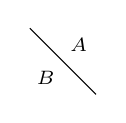
\begin{tikzpicture}[scale=0.7]
	\draw (-.6,.6) -- (.6,-.6);
	\node at (-.3,-.3) {$\ham_{B}$};
	\node at ( .3, .3) {$\ham_{A}$};
\end{tikzpicture} &|\phi_1 \rangle, & |\phi_2 \rangle, &\ldots \\[5pt] \hline \\[-5pt]
|\chi_1\rangle &|\phi_1\rangle \otimes|\chi_1\rangle &\ldots\\
|\chi_2\rangle &.\\
. &.\\
.\\
.
\end{array}
\end{equation*}

\end{itemize}

%20.05.19

\subsubsection{\emph{Bemerkungen:}}

\begin{enumerate}
	\item[(1)] war der Rest der letzten Vorlesung über Tensorräume
	\item[(2)] Für einen Operator der Form $ O = A + B + C $ mit $ A|a\rangle = a | c \rangle \dots $ gilt:
	%
	%
	%
	\setcounter{equation}{59}
	%
	%
	%
	\begin{equation}
	O | a, b, c \rangle = (a + b + c) |a, b, c \rangle
	\end{equation}
	
	\subsubsection{\emph{Beispiel:}}
	
	Helium-Atom ohne e-e-Wechselwirkung\\[5pt]
	Anreguns:
	\begin{equation*}
	H_{He} = H_{Z=2}^{(1)} + H_{Z=2}^{(2)} = -\frac{1}{2n_1^2} - \frac{1}{2n_2^2}
	\end{equation*}
	Die $ H_{Z=2} $ Terme sind klassische Wasserstoffähnliche Atome. 
\end{enumerate}
Allgemeinster (Zustands-) Vektor im bipartitem Hilbertraum $ \ham = \ham_{A} \otimes \ham_{B} $
%
%
%
\setcounter{equation}{56}
%
%
%
\begin{equation*}
|\psi \rangle = \sum_{jk} c_{jk} | \varphi_j \rangle \otimes | \chi_{k} \rangle
\end{equation*}
$ |\varphi_j \rangle $ und $ |\chi_{k}\rangle $ sind beliebig und nicht notwendig Basisvektoren !
\begin{equation*}
| \psi \rangle \neq | \varphi \rangle \otimes | \chi \rangle \quad , \quad \forall |\varphi \rangle \in \ham_{A} , |\chi \rangle \in \ham_{B}
\end{equation*}
heißt \textbf{verschränkt} oder \textbf{nicht-separabel} $ \Big| $ entangled or non-entangled.\\[5pt]
Wichtiges Hilfsmittel zur Charakterisierung des Verschänkungsgehalts bipartiter Systeme:\\
\textbf{Schmidt-}\textbf{Zerlegung}
$ \forall | \psi \rangle \in \ham = \ham_{A} \otimes \ham_{B} $ gibt es eine ONB $ \left\{ |j_{A}\rangle \right\}, \left\{ |j_{B}\rangle \right\} $ von $ \ham_{A} $ und $ \ham_{B} $, sowie Koeffizienten: $$ \lambda_j \in \mathbb{R}_{0}^{+}, \sum \lambda_j^2 = 1 $$
%
%
%
\setcounter{equation}{60}
%
%
%
\frbox{Schmidt-Zerlegung}{
\begin{equation}
|\psi \rangle = \sum_{j} \lambda_j | j_{A} \rangle \otimes | j_{B} \rangle
\label{2 61}
\end{equation}}
\noindent
Dies ist eine erhebliche Vereinfachung gegenüber II.49 und II.57\\[10pt]
%
%
%
% correct eqrefs oben
%
%
%
\textbf{Bisher:} Einbettung der Elemente der Faktorräume in den Tensorraum.\\[5pt]
\textbf{Jetzt:} umgekehrte Richtung - lassen sich $ |\psi\rangle $ aus $ \ham $ in eindeutiger Weise mit Zuständen der Faktorräume identifizieren ?\\[5pt]
Sei $ |\psi\rangle \in \ham $, dann ist gemäß \eqref{2 9} der Projektor auf $ |\psi\rangle $ durch:
\begin{equation}
P_{|\psi\rangle} \overset{\eqref{2 9}}{=} |\psi\rangle \langle \psi | \overset{\eqref{2 61}}{=} \sum_{j j'} \lambda _j \lambda _{j'} | j_{A}\rangle \langle j_{A}' | \otimes | j_{B} \rangle \langle j_{B}' |
\label{2 62}
\end{equation}
Zunächst nehmen wir an, $ |\psi\rangle $ besitze nur einen nichtverschwindenden Schmidt-Koeffizienten, d.h. $ \lambda_j = \delta_{jk} $, womit folgt:
\begin{equation}
| \psi \rangle \langle \psi | = | k_{A} \rangle \langle k_{A} | \otimes | k_{B} \rangle \langle k_{B} |
\label{2 63}
\end{equation}
Bilden wir die \textbf{partielle Spur} dieses Projektionsoperators über eine vollständige Basis von $ \ham_{B} $, so erhalten wir:
\begin{equation*}
\begin{aligned}
\custo{\leftarrow}{\tx{tr}_{B}}{\tx{``trace''}} |\psi \rangle \langle \psi| &= \custo{\leftarrow}{\tx{Sp}_{B}}{\tx{,,Spur``}} | \psi \rangle \langle \psi| = \sum_{m} \phantom{\rangle}_{B}\langle m|\psi \rangle \langle\psi|m\rangle_{B} \\
&= \sum_{m} \phantom{|}_{B}\langle m | \bigg[ | k_{A} \rangle \langle k_{A} | \otimes | k_B \rangle \langle k_B| \bigg] |m \rangle_{B} \\
& \hspace{-7.5pt} \overset{\eqref{2 63}}{=} \sum_{m} |k_{A} \rangle \langle k_{A} | _{B}\langle m|k_{B}\rangle \langle k_{B}| m \rangle_{B} \\
&= |k_{A} \rangle \langle k_{A}| \sum_{m} \langle k_{B} | m \rangle_{B} \langle m | k_B \rangle \\
&= |k_{A} \rangle \langle k_{A} | \langle k_B | \ub{\sum_{m} | m \rangle_{B} \phantom{|}_{B} \langle m | }_{\mathclap{= \mathbbm{1} : \tx{ Vollständigkeit !}}} | k_{B} \rangle = | k_A\rangle \langle k_A| \ub{\langle k_B| k_B\rangle}_{\overset{\eqref{2 61}}{=} 1}\\
&= | k_{A} \rangle \langle k_{A} |
\end{aligned}
\end{equation*}
wobei $ _{B}\langle m | $ und $ | m \rangle_{B} $ ONB-Vektoren aus $ \ham_{B} $ sind.\\[5pt]
Es gilt also:
\begin{equation}
\tx{tr}_{B} |\psi \rangle \langle\psi | = | k_A \rangle \langle k_A |
\label{2 64}
\end{equation}
Dies liefert also eine eindeutige Zuordnung zwischen $ |\psi\rangle \in \ham $ (mit der Voraussetzung $ \lambda_j = \delta_{jk} $ !!!) und $ |k_{A}\rangle \in \ham_{A} $ (nach Ausspuren der $ \ham_{B} $-Komponente von $ |\psi \rangle $).\par
Völlig analog gilt:
\begin{equation}
\tx{tr}_{A} | \psi \rangle \langle \psi | = | k_{B} \rangle \langle k_{B} |
\label{2 65}
\end{equation}

\subsubsection{Interpretation von (II.64, II.65)}

Verzicht auf die in den Basiszuständen des Faktorraums, über den gespurt wird, kodierte Information bringt \textbf{keinen} Informationsverlust bzgl. des in den Basiszuständen des verbleibenden Faktorraums eingeschriebene Struktur.\par
Die Situation verändert sich grundlegend, wenn wir mehr als einen nichtverschwindenden Schmidt-Koeffizienten $ \lambda_j $ in \eqref{2 61} zulassen:\par
Mit \eqref{2 62} erhält man für die Spur über $ \ham_{B} $:
\begin{equation}
\begin{aligned}
\tx{tr}_{B}|\psi \rangle \langle \psi | \hspace{7.5pt} & \hspace{-7.5pt}\overset{\eqref{2 62}}{=} \sum_{m} \sum_{jj'} \lambda_{j} \lambda_{j'} | j_{A} \rangle \langle j_{A}' | \ub{_{B} \langle m | j_{B} \rangle}_{\delta_{mj}} \ub{\langle j_{B}' | m \rangle_{B}}_{\delta_{mj'}} \\
&= \sum_{m} \lambda_m^2 | m_a \rangle \langle m_a | \eqdef \rho_{A} = \tx{ reduzierte Dichtematrix}
\end{aligned}
\label{2 66}
\end{equation}
mit $ |\psi \rangle = $ Zustand(-s-Vektor) und $ \rho = $ Zustand.\\[5pt]
Dies ist ein diagonaler Operator auf $ \ham_{A} $, mit Eigenwerten $ \lambda_m^2 < 1 $. Da aber jeder Projektor $ | \varphi \rangle \langle \varphi | $ auf einen beliebigen Zustand $ |\varphi \rangle \in \ham_{A} $ Eigenwerte $ 0 $ und $ 1 $ hat, lässt sich $ \tx{tr}_{B} |\psi \rangle \langle \psi | $ im allgemeinen \textbf{nicht} mit einem Zustandsvektor in $ \ham_{A} $ identifizieren!
\begin{equation}
\rmbox{
\begin{aligned}
\tx{tr}_{B} | \psi \rangle \langle \psi | &= \rho_{A} \\
\tx{tr}_{A} | \psi \rangle \langle \psi | &= \rho_{B}
\end{aligned}}
\label{2 67}
\end{equation}
Dabei ist $ \rho $ der \textbf{reduzierte/r Dichtematrix -operator} oder \textbf{statistischer Operator}.\\[5pt]

%21.05.19

\noindent
Partielle Spurbildung über $ \ham_{A} $ oder $ \ham_{B} $ führt i.a. (d.h. für beliebige Verteilung der Schmidt-Koeffizienten von $ |\psi\rangle $) auf operatorwertige Objekte der Form \eqref{2 66}, die nur für separable $ |\psi\rangle $ projektorwertig sind.\par
Dichtematrizen haben folgende Eigenschaften:
\begin{equation}
\begin{aligned}
\rho_{A}^{\dagger} &= \rho_{A} \\
\tx{tr}_{A} \rho_{A} \hspace{7.5pt} & \hspace{-7.5pt} \underset{\substack{\eqref{2 61}\\\eqref{2 66}}}{=} 1 = \tx{tr}_{A} \tx{tr}_{B} |\psi \rangle \langle \psi| \\
\tx{tr} \rho_{A}^2 &\le 1 \\
\rho_{A} &\ge 0
\end{aligned}
\label{2 68}
\end{equation}
Zur letzten Eigenschaft gilt: $ \tx{d.h. $ \rho_{A} $ hat nichtneg. EW} \quad \rho_{A} \tx{ positiver Operator} $.\\[5pt]
Wegen $ \sum \lambda_{m}^2 = 1 $ und $ \lambda_m \in \mathbb{R}_{0}^{+} $ gilt, dass $ \tx{tr} \rho_{A}^2 = 1 $ genau dann, wenn:
\begin{equation}
\rho_{A} = |\varphi \rangle \langle \varphi| \quad \tx{mit} \quad |\varphi\rangle \in \ham_{A}
\label{2 69}
\end{equation}
Gilt \eqref{2 69}, so bezeichnet man $ \rho_{A} $ als ,,\textbf{reinen Zustand}``, der m.a.W. dadurch gekennzeichnet ist, dass er mit einem Zustands-Vektor identifizierbar ist. Andernfalls heißt $ \rho_{A} $ ,,\textbf{gemischter Zustand}`` ($ \Leftrightarrow \tx{tr} \rho_{A}^2 \lneq 1 $).\par
Motivation der Begrifflichkeit durch Wahl einer bestimmten Darstellung (d.h. in vorgegebener Basis) 
\begin{equation}
\begin{aligned}
\rho_{A} &= | \varphi \rangle \langle \varphi | = \left( \sum_{j} c_j |j\rangle \right) \left(\sum_{l} c_l^{*} \langle l | \right) = \sum_{jl} c_j \cdot c_l^{*} |j\rangle\langle l|\\
&= \begin{pmatrix}
|c_1|^2 & c_1 c_2^{*} & c_1 c_3^{*} & \dots \\[3pt]
c_1^{*} c_2 & |c_2|^2 & c_2 c_3^{*} & \dots \\[3pt]
c_1^{*} c_3 & c_2^{*} c_3 & |c_3|^2 \\
\vdots & \vdots & & \ddots
\end{pmatrix}
\end{aligned}
\label{2 70}
\end{equation}
Diagonalisierung führt (da $ \rho_{A} $) ein Projektor ist) auf:
\begin{equation*}
\begin{pmatrix}
1 & 0 & 0 & \dots \\
0 & 0 & 0 & \dots \\
0 & 0 & 0 \\
\vdots & \vdots & & \ddots
\end{pmatrix}
\end{equation*}
Dagegen wissen wir wegen \eqref{2 66}, dass ein gemischter Zustand die Diagonalform:
\begin{equation}
\begin{pmatrix}
|c_1|^2 & 0  & \dots \\
0 & |c_2|^2  & \dots \\
\vdots & \vdots & \ddots
\end{pmatrix}
\label{2 71}
\end{equation}
hat, also \textbf{nicht} in die Form von \eqref{2 70} überführt werden kann (bei \eqref{2 71} mindestens 2 Diagonaleinträge $ \neq 0 $).\par
Reminiszenz an Kapitel \ref{Isection1} (Doppelspalt) und \ref{Isection2} dort: Die Interferenzterme dort werden in \eqref{2 70} gerade durch die Nebendiagonalelemente bestimmt. Die relevante Information über die Interferenzfähigkeit des Systems ist den ,,\textbf{Kohärenzen}``
\begin{equation*}
c_ic_j^* = |c_i| |c_j| e^{i(\varphi_i - \varphi_j)}
\end{equation*}
in der vorgegebenen Basis eingeschrieben.


%T1
\hft


\noindent
Die Diagonalelemente der Dichtematrix heißen auch ,,\textbf{Populationen}`` (Wkt. für sich klassisch ausschließende Alternativen). Das Abklingen (d. Ausdämpfen) der Nebendiagonalelemente/Kohärenzen in einem dynamischen Prozess heißt ,,\textbf{Dekohärenz}``.\par
Da man mit dem Verschwinden des Interferenzterms die Phänomenologie klassischer Teilchen am Doppelspalt gewinnt, vermittelt Dekohärenz der \textbf{quanten-klassischen Übergang}.\\[5pt]
\lcom{Interessantes Paper zu Buckyballs auf ILIAS}